\documentclass[10pt,a4paper,ngerman]{scrartcl}
\usepackage[utf8]{inputenc}
\usepackage[ngerman]{babel}
\usepackage[T1]{fontenc}
\usepackage{amsmath}
\usepackage{amsfonts}
\usepackage{amssymb}
\usepackage{makeidx}
\usepackage{graphicx}
\usepackage{epstopdf}
\usepackage[onehalfspacing]{setspace}
\usepackage{array}
\usepackage{upgreek}
\usepackage{float}
\usepackage{csquotes}
\usepackage{chemformula}
\usepackage{chemgreek}
\usepackage{chemmacros}
\chemsetup{modules=all}
\usepackage{tikz}
\usepackage{siunitx}
\sisetup{locale = DE,per-mode = symbol}
\usepackage{esvect}
\usepackage{geometry}
\usepackage{pdfpages}
\usepackage[font=small]{caption}
%\usepackage[version=4]{mhchem}
\usepackage[backend=biber, style=chem-angew]{biblatex}
\addbibresource{Ionische.bib}
\usepackage{tabularx, booktabs, multirow}
\usepackage[pdfborder={0 0 0}]{hyperref}
\usepackage{scrlayer-scrpage}%Header für die KOMA-script -Klasse
%\usepackage{hyperref}
\usepackage{pgfplots}
\usepackage{textgreek}


\newcommand{\tildenu}{{\fontencoding{LGR}\selectfont\accperispomeni\textnu}}
\captionsetup{format=plain}
\chemsetup[phases]{pos=sub}
\chemsetup[redox]{pos=top}
\chemsetup[redox]{align=center}
%\chemsetup[redox]{explicit-sign=true}
%\chemsetup[redox]{roman=false}
\newcommand{\celsius}{^{\circ}\mathrm{C}}
\parindent0pt
\sloppy
\DeclareChemPhase{\s}{s}
\DeclareChemPhase{\l}{l}
\DeclareChemPhase{\g}{g}
\renewcaptionname{ngerman}{\figurename}{Abb.}
\renewcaptionname{ngerman}{\tablename}{Tab.}
\geometry{bottom=100pt} \geometry{top=80pt}
\newcommand{\m}{\mathrm{m}}
\newcommand{\K}{\mathrm{K}}
\newcommand{\J}{\mathrm{J}}
\newcommand{\gr}{\mathrm{g}}
\newcommand{\kg}{\mathrm{kg}}
\newcommand{\mol}{\mathrm{mol}}
\newcommand{\Pa}{\mathrm{Pa}}
\newcommand{\ad}{\mathrm{ad}}
\newcommand{\de}{\mathrm{de}}
\newcommand{\gmol}{\mathrm{\frac{g}{mol}}}
\newcommand{\JKmol}{\mathrm{\frac{J}{K \cdot mol}}}
\newcommand{\kgmss}{\mathrm{\frac{kg}{m \cdot s^2}}}
\newcommand{\loge}{\mathrm{ln}}


\begin{document}
\begin{titlepage}
	\vspace*{2,5cm}
	\begin{center}
		\begin{LARGE}
			\textbf{Polymer Chemie}\\
			\textbf{Ionische Polymerisation}\\
		\end{LARGE}
		\vspace{1cm}
		\textbf{Universität Stuttgart}\\
		\vspace*{1,5cm}
		\begin{tabular}{lp{7,5cm}l}
			Author 1:     &Laurens Viehoff\\
            Author 2:     &Felix Roth\\   
			E-Mail 1:      &st183688@stud.uni-stuttgart.de\\
            E-Mail 2:      &st188157@stud.uni-stuttgart.de  \\
			Student-ID 1: & 3676761   \\ 
            Student-ID 2: & 3711192 \\ \\
			Assistentin:  &   \\ \\ 
		\end{tabular}
	\end{center}

    
\end{titlepage}
\thispagestyle{empty}
\renewcommand{\thepage}{\arabic{page}}
\newpage
\tableofcontents
\setcounter{page}{1}
\renewcommand{\thepage}{\arabic{page}}
\newpage

 
\section{Theorie}

	Der kerngedanke der Ionischen Polymerisation ist das bilder Polymerkette durch anlagerung der Monomere an 
	ein Makroanion oder ein Makrokation. Die Ladung des Makroions entscheidet hierbei darüber ob es sich um eine 
	Anionische- oder eine kationische-Polymerisation handelt. Diese Ladung der Endgruppe kann durch unterschiedliche dinge
	wie Lösemittel, Gegenionen, Temperatur und druck beeinflusst werden \ref{Ladungsggw}.

		\begin{figure}[H]
			\centering
			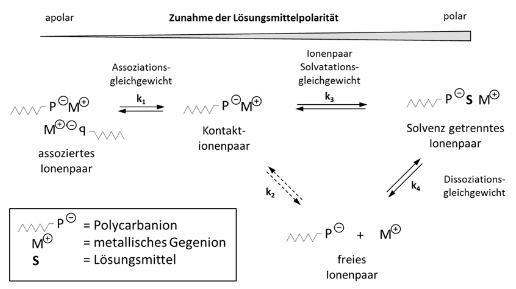
\includegraphics{Bilder/Lösemitteleinfluss.png}
			\caption{Die Abbildung zeigt den Einfluss des Lösemittels auf das gleichgewicht der Ionen im falle der Anionischen Polymerisation von Styrol. \cite{polyskript}}
			\label{Ladungsggw}
		\end{figure}

	Die Stärke dieses Ions nimmt dabei sehr goßen einfluss auf die Wachstumsgeschwindigkeit. 
	So sind gebundene Ionenpaare langsamer in ihrem Wachstum als freie Ionen.\\
	
	Wird die Ionische Polymerisation mit z.B. der radikalischen Polymerisation verglichen. Wird deutlich,
	dass bei der Ionischen Polymerisation die möglichkeit besteht, diese lebend durchzuführen. 
	Da die aktiven Zentren nicht miteinander reagieren können. Somit kann die Polymerisation theoretisch
	endlos aufrecht erhalten werden, bzw. sie kann durch erneute zugabe von Monomer weitergeführt werden.
	Diese wird nur durch zugeben einer Brönsted-Base abgebrochen es wird auch von "abtöten" gesprochen.

	\subsection{Ablauf der lebenden anionische Polymerisation}

		Die lebende anionische Polymerisation kannn wie bei der radikalischen Polymerisation in drein Teile geteilt werden.\\
		Der erste Schritt ist die Initiierung. Hierfür werden bei der Ionischen Polymerisation Brönsted-Säuren und Brösnsted Basen verwendet.
		Hierbei gilt die Regel je weniger elekrophil das Zentrum aktiviert ist umso stärker muss die Säure oder Base sein.
		Beispiele für solche Initiatoren sind Alkalimetalle, Alkylverbindungen und Alkalimetallnaphthalide \cite{polyskript}.
		Im Rahmen dieses Versuchs wurde \textit{sec}-BuLi verwendet. Dabei reagiert dieses nach folgendem Prinzip:

			\begin{figure}[H]
				\centering
				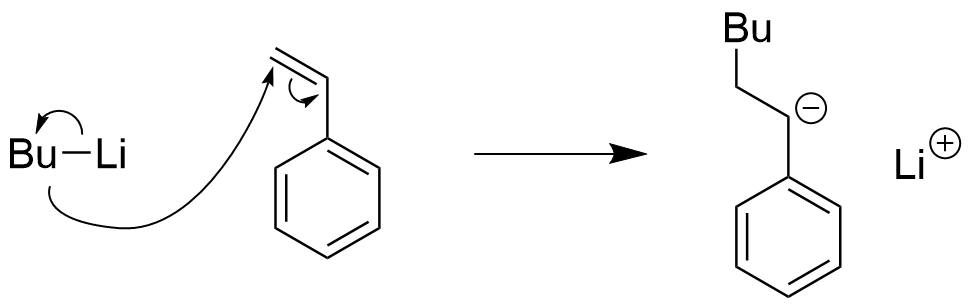
\includegraphics[scale = 0.35]{Bilder/Initiierung.png}
				\caption{Die Abbildung zeigt den Initiatorschritt von Styrol mit BuLi.}
				\label{Initiierung}
			\end{figure}

		Eine weitere Methode die Reaktion zu Initiieren ist durch Naphthalin mit einem Alkalimetall. 
		Hierbei wird zuerst ein Radikalanion gebildet welches anschließend seine ladung sowie das Radikal an das Monomer (unserem Fall Styrol) abgibt.
		das hierraus entstandene Radikalanion Monomer rekombiniert und hat anschließend zwei aktive anionische enden.

			\begin{figure}[H]
				\centering
				
\includegraphics[scale = 0.6]{Bilder/NaphthalinStarter.png}
				\caption{Die Abbildung zeigt den Initiatorschritt von Styrol mittels der Alkalimetallnaphthaliden.\cite{polyskript}}
				\label{NaphthalinStarter}
			\end{figure}
		
		
		Nach der Initiierung findet das Kettenwachstum Statt auch gezeigt in Abb. [\ref{Wachstum}].

			\begin{figure}[H]
				\centering
				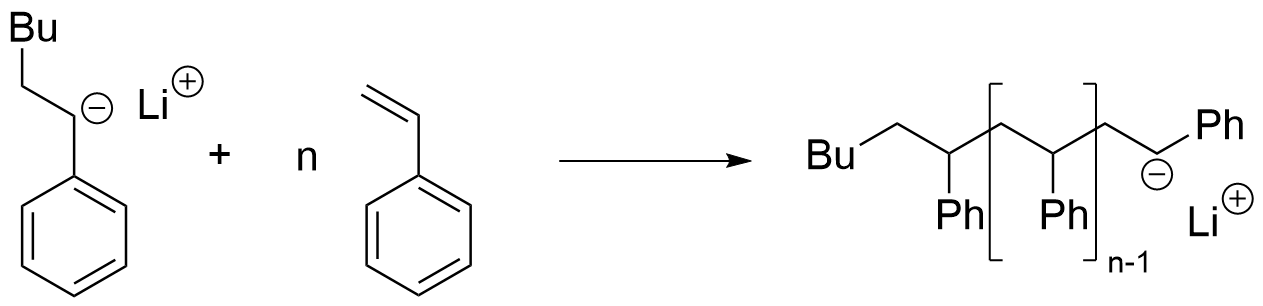
\includegraphics[scale = 0.3]{Bilder/Wachstum.png}
				\caption{Die Abbildung zeigt den Allgemeinen Wachstumsschritt anhand des Peispiels von Styrol.}
				\label{Wachstum}
			\end{figure}


		Dieses Wachstum hat am meisten einfluss auf die Reaktionskinetik der Polymerisation. 
		So ergibt sich der Polymerisationsgrad P$_\text{n}$ wie folgt:

			\begin{equation}
				\bar{\text{P}}_\text{n} = \frac{[M]_0 - [M]_t}{[I]}
				\label{Polymerisationsgrad}
			\end{equation}

		Hierbei ist [M]$_0$ die Monomerkonzentration zu beginn (t=0), [M]$_\text{t}$ ist die Monomerkonzentration zu dem Zeitpunkt t
		und [I] ist die Initiatorkonzentration. Aus P$_\text{n}$ lässt sich der Polydispersitätsindex (PDI) berechnen. 
		Er beschreibt die Poisson-Verteilung der Molmassenverteilung und ist durch folgende Gleichung gegeben:

			\begin{equation}
				PDI = \frac{\bar{P}_w}{\bar{P}_n} = \frac{\bar{M}_w}{\bar{M}_n} = 1 + \frac{1}{\bar{P}_n}
			\end{equation}
			
		Hierbei ist $\bar{M}_w$ das Gewichtsmittel der Molmassenverteilung, $\bar{M}_n$ das Zahlenmittel der Molmassenverteilung,
		$\bar{P}_n$ der Zahlenmittlere Polymerisationsgrad und $\bar{P}_w$ der Gewichtsmittlere Polymerisationsgrad. 
		Dabei gilt, dass synthetische Polymere mit einem undendlichen Polymerisationsgrad den PDI von 1 haben.
		Dabei ist wichtig, dass dies lediglich ein theoretischer Wert ist und nicht realisierbar ist.\\\\

		Zuletzt findet der Abbruch der Polymerisation statt. 
		Dabei wird nur von nicht lebenden Polymerisation gesprochen da die lebendende Polymerisation keinen Abbruch besitzt.
		Die Carbanionen werden in der Regel mit schwachen Säuren wie Methanol oder Wasser abgebrochen.
		Hierbei findet eine große beeinflussung auf die finalen eigenschaften des Polymers statt. 
		Da durch verwendung von unterschiedlichen Abbruchreagenzien zu unterschiedlichen Endgruppen führt.
		So wird beispielsweiese durch Abbrechen der Reaktion mit \ch{CO2} eine Carboxylgruppe die endgruppe [\ref{Abbruch}].

			\begin{figure}[H]
				\centering
				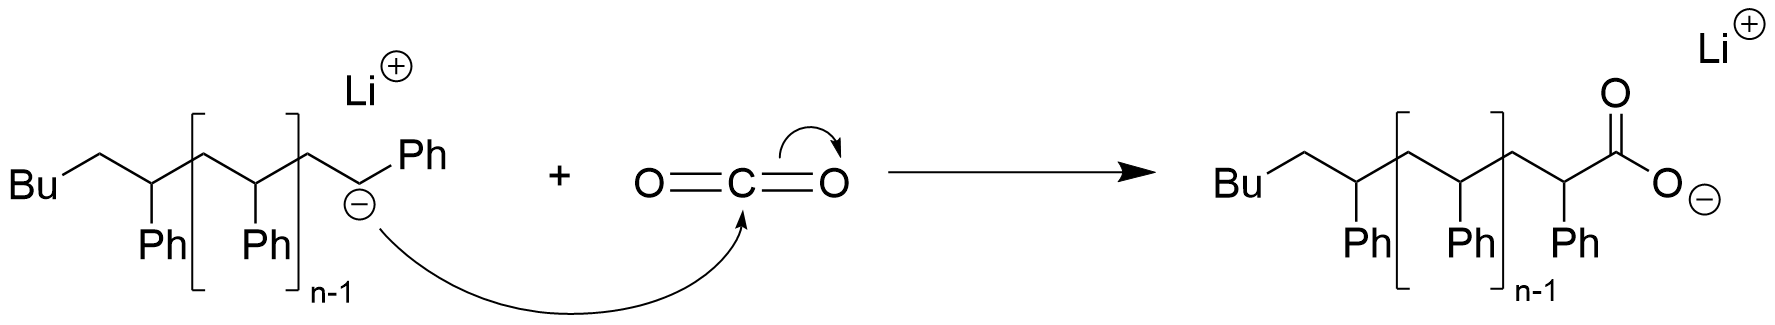
\includegraphics[width = \textwidth]{Bilder/Abbruch.png}
				\caption{Die Abbildung zeigt den Mechanistischen Abbruch der Polymerisation mittels \ch{CO2}.}
				\label{Abbruch}
			\end{figure}

			

\section{Durchführung}

	Innerhalb des Gesamten Versuches wurde unter schlenk bedingungen gearbeitet.\\
	In einem Dreihalskolben mit glasummantelten Rührfisch wurde Toluol (\SI{40}{ml}) vorgelegt und auf 50°C hochgeheizt.
	Anschließend wurde Styrol (\SI{3}{ml}) und zuletzt AIBN (\SI{1}{ml}) zugegeben.
	Nach 30 min wurde Isopren (\SI{2}{ml}) zugegeben und weitere 2 h gerührt. 
	Zur terminierung der Reaktion wurde Methanol (\SI{0,5}{ml}) zu der lösung gegeben, 
	und das Polymer wurde in ca. \SI{400}{ml} gekühltem Methanol gefällt und Im Vakuumtropckenschrank getrocknet.
	


\section{Auswertung}

	

\printbibliography

\end{document}